\chapter{\label{app:genLanger}Generalized Kramers-Langer rates}
This appendix provides a detailed derivation of the generalized Kramers-Langer-Theory presented
in \SEC{tsr}. The derivation is kept general and we refer the reader to \SEC{tsr} or the publication reprinted
in \SEC{tsr_rotor} for a concrete application. In 1969, J.~Langer published a generalization of the celebrated
Kramers' formula for thermally activated escape from a one-dimensional potential well to barrier 
crossing processes in many dimensions \cite{Langer_APNY_69}. 
A concise and clear derivation of this formula can be found in \REF{Haenggi_RevModPhys_90}.
The Langer formula, as presented by \citeauthor{Haenggi_RevModPhys_90}\cite{Haenggi_RevModPhys_90}, assumes a constant
mobility matrix in the relevant saddle point region. However, in many systems and especially in those described by
generalized coordinates, this assumption cannot be made. 
Here, we seek to incorporate the configuration dependence of the mobility matrix into the Langer formula. 

The escape rate out of a meta-stable potential well separated from a stable region by a unique
saddle point is given by ratio of the probability current over the saddle point and the population 
inside the well. The evolution of the probability density $\PD(\{\eta\})$ is determined by the 
Fokker-Plank equation (FPE) $\partial_t \PD(\{\eta\},t)=-\nabla\cdot\mathbf{j}(\{\eta\},t)$, where the
flux density $\mathbf{j}(\{\eta\},t)$ is given by
\begin{equation}
\label{eq:FPE}
%\frac{\partial \PD(\{\eta\})}{\partial t} = \partial_i \left[\Mobc_{ij}\frac{\partial U(\{\eta\})}{\partial \PD_j}+\kT\Mobc_{ij} \partial_j \right]\PD(\{\eta\}),
j_i (\{\eta\},t)= -\left[\Mobc_{ij}\frac{\partial V(\{\eta\})}{\partial \eta_j}+\kT\Mobc_{ij} \partial_j \right]\PD(\{\eta\},t),
\end{equation}
The matrix $\Mob$ is the mobility matrix which in general depends on the configuration 
$\{\eta\}$ and $V(\{\eta\})$ is the potential energy.
We consider only the purely diffusive case and neglect any symplectic contributions to $\Mob$, 
which is justified since the applications in mind are completely overdamped.
Let us now assume that particles are injected into the meta-stable well at a constant rate and removed
from the stable region. In this case, $\PD(\{\eta\})$ tends to a steady state, with a distribution that is very close
the equilibrium distribution inside the meta-stable well, and which vanishes beyond the saddle where particles are
removed. This steady state distribution carries a probability flux density out of the meta-stable well into the
region where particles are removed. Obviously, the total flux integrated over any surface separating the insertion site from the absorbing boundary is equal to the rate of particle insertion. The non-trivial task 
is to relate this flux to the population inside the meta-stable well, \emph{i.e}~the number of 
particles that accumulate before the steady state is attained. To this end, we solve the FPE in the vicinity
of the saddle point where the probability flux is concentrated to a narrow channel, and
match this solution to the approximate pseudo-equilibrium solution inside the meta-stable region.
%The mobility matrix relates the forces and the spatial inhomogeneities to the the probability flux.
The size of the relevant saddle point region is determined by the curvature of the potential 
energy at the saddle point. Within this region, we can expand the potential 
energy, resulting in the simple FPE
\begin{equation}
\label{eq:steadyFPE}
\partial_i \left[\Mobc_{ij}\UHessc_{jk}\eta_k+\Mobc_{ij}\kT \partial_j \right]\PD(\{\eta\}) =0,
\end{equation}
where $\UHess$ is the Hessian of the energy near the saddle point.
Since we need to match the solution near the saddle point to the equilibrium distribution inside the well,
we rewrite $\PD(\{\eta\})$ in the form 
$\PD(\{\eta\})=\PD_{eq}(\{\eta\})\Ansatz(\{\eta\})$, where $\PD_{eq}(\{\eta\})$ is the equilibrium distribution. 
Using this ansatz we can decompose the above equation into the equations
\begin{equation}
\begin{split}
\label{eq:flux}
\partial_i \Ansatz(\{\eta\}) \left[\Mobc_{ij}\UHessc_{jk}\eta_k+\kT \Mobc_{ij}\partial_j \right]\PD_{eq}(\{\eta\})=0\\
\partial_i \PD_{eq}(\{\eta\})\kT \Mobc_{ij} \partial_j \Ansatz(\{\eta\})=0,
\end{split}
\end{equation}
the first of which is trivially fulfilled since it includes the current of $\PD_{eq}(\{\eta\})$. 

If the mobility matrix changes significantly inside the saddle point region, its variation has to be taken into account. 
Here, we seek to incorporate this variations by expanding the mobility matrix about the saddle point
and calculate the correction to the rate. 
%To calculate this flux, we expand the 
%the potential landscape and the mobility matrix around the saddle point and solve the FPE
%in a harmonic approximation for a steady state solution. It has to be taken care that the expansion of the
%mobility matrix is reasonable inside the relevant saddle point region and in particular does not become negative.
Each entry of the mobility matrix $\Mob$ can be expanded separately as
\begin{equation}
\Mobc_{ij}=\Mobc_{ij}^0+\frac{\partial \Mobc_{ij}}{\partial \eta_k}\eta_k + \frac{1}{2}\frac{\partial^2 \Mobc_{ij}}{\partial \eta_k\partial \eta_l}\eta_k\eta_l+\mathcal{O}(\eta^2),
\end{equation}
where $\eta_k$ are the deviations from the saddle.
For symmetry reasons the linear dependence on $\eta_k$ will often vanish and for the moment we will drop 
the linear term. In short, we have 
$\Mobc_{ij}=\Mobc_{ij}^0+\frac{1}{2}\MobHessc_{kl}^{ij}\eta_k\eta_l$
with the symmetric matrix $\mathbf{A}^{ij}$ for each entry of $\Mob$. 
Inserting this expansion into \EQ{flux} yields
\begin{equation}
\begin{split}
\label{eq:flux_ansatz}
\left[-\UHessc_{ik}\Mobc_{ij} + \kT \NIDcoeff_{jk}\right]\eta_k\partial_j \Ansatz(\{\eta\})+
\kT \Mobc_{ij} \partial_i \partial_j \Ansatz(\{\eta\})=0\;,
\end{split}
\end{equation}
where the matrix $\NID$ is defined by 
\begin{equation}
\partial_i \Mobc_{ij}= \frac{1}{2}\sum_{i} \left(\delta_{il}\MobHessc_{lk}^{ij}\eta_k+\delta_{ik}\MobHessc_{lk}^{ij}\eta_l\right)=\sum_{i}\MobHessc_{ik}^{ij}\eta_k=\NIDcoeff_{jk}\eta_k.
\end{equation}
$\NIDcoeff_{kl} \eta_l$ is the noise induced drift due to the configuration dependence of the 
mobility matrix and which is absent in the conventional Langer theory. 
To solve this equation, we employ the ansatz \cite{Haenggi_RevModPhys_90}
\begin{equation}
\Ansatz(\{\eta\})=\frac{1}{\sqrt{2\pi\kT}}\int_u^{\infty}\exp(-\frac{z^2}{2\kT}) dz,
\end{equation}
where the lower integration boundary depends on $\eta_k$ via $u=\sum_i \Sepc_i\eta_i$, where the 
vector $\Sep$ is to be determined by \EQ{flux_ansatz}.
This function interpolates smoothly between one inside the meta-stable region and
tends to zero beyond the saddle point and therefore automatically satisfies the matching condition.
Inserting this ansatz into \EQ{flux_ansatz} yields, after a bit of algebra
\begin{equation}
\label{eq:eigenvectoreq}
\begin{split}
\left[\Sepc_j(-\Mobc_{ji}\UHessc_{ik}  + \kT \NIDcoeff_{jk}) -
\Sepc_i \Mobc_{ij} \Sepc_j\Sepc_k\right]\eta_k=0
\end{split}
\end{equation}
Since this equation should hold for any set $\eta_k$, the term in brackets itself has to vanish.
%\begin{equation}
%\label{eq:eigenvectoreq}
%\begin{split}
%(-\Mobc_{ji}\UHessc_{ik} + \kT \NIDcoeff_{jk}) \Sepc_j-(\Sepc_i\Mobc_{ij} \Sepc_j)\Sepc_k=0
%\end{split}
%\end{equation}
\EQ{eigenvectoreq} is equivalent to equation 4.71 in \REF{Haenggi_RevModPhys_90}, but includes the 
additional drift $\kT \NIDcoeff_{jk}\eta_k$ induced by the configuration dependence of $\Mob$. In this equation,
the explicit configuration dependence of $\Mobc_{ij}=\Mobc_{ij}^{0}+\frac{1}{2}\MobHessc_{kl}^{ij}\eta_k\eta_l$
is of second order in $\eta_k$ and can therefore be neglected. After substituting $\Mobc_{ij}^{0}$
for $\Mobc_{ij}$, \EQ{eigenvectoreq} is an eigenvector equation 
for $\Sep$, which determines $\Sep$ to be a left eigenvector of $-\Mobc_{ji}^0\UHessc_{ik}  + \kT \NIDcoeff_{jk}$. 
The norm of $\Sep$ is fixed by the condition $\lambda=\Sepc_i\Mobc_{ij}^0 \Sepc_j$, where $\lambda$ is the
eigenvalue corresponding to the eigenvector $\Sep$. In particular, this condition requires $\lambda$ 
to be positive. The necessity of the noise-induced drift term is illustrated in \FIG{separatrix}, where the stochastic separatrix is 
plotted for different temperatures. The vector $\Sep$ has an appealing interpretation:
$\Sep$ is perpendicular to the stochastic separatrix, \emph{i.e.}~the hyperplane where the probabilities
to relax either into the meta-stable or stable region are both equal to 0.5. The right eigenvector to the same eigenvalue
points into the direction of the diffusive flux at the transition state \cite{Berezhkovskii_JChemPhys_05}. The right 
and left eigenvectors coincide if $\Mob$ is diagonal.
%If the $\NIDcoeff_{jk}$ vanish, the latter implies 
%$\Sep e^{-1}_{ij}\Sepc_j=-\frac{1}{\lambda}\Sepc_l \Mobc_{lk}\UHessc_{ki}e^{-1}_{ij}\Sepc_j=-1$.
%For non zero $\NIDcoeff_{jk}$, one has $\Sepc_i e^{-1}_{ij}\Sepc_j=-1 + \frac{kT}{\lambda}\Sepc_l \NIDcoeff_{li}e^{-1}_{ij}\Sepc_j$.
%This correction term will reappear later on.
\begin{figure}
\centering
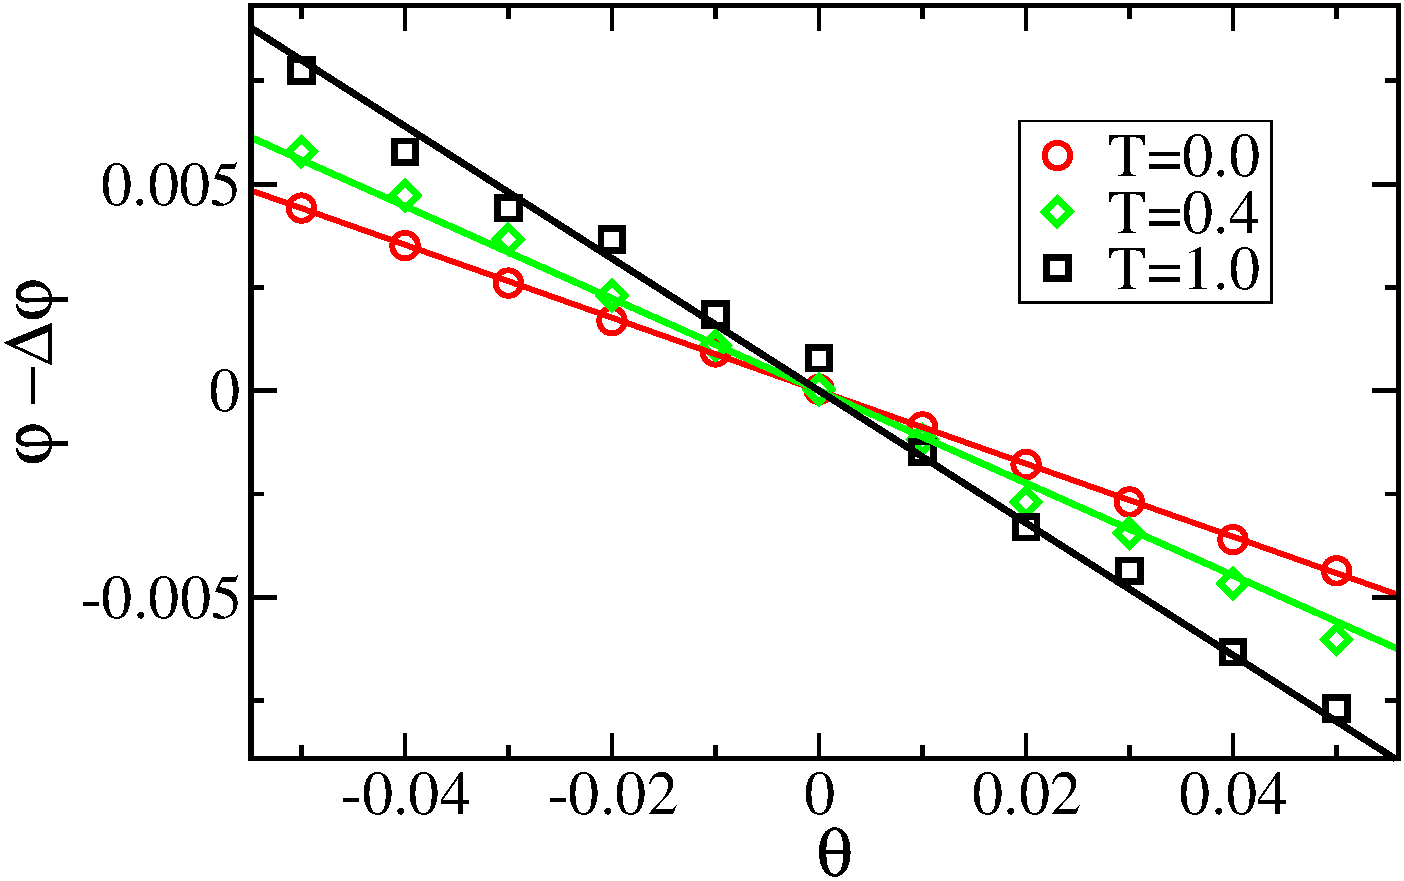
\includegraphics[width=\halffigure]{\FIGPATH/Figures_AppendixB/separatrix}
\caption[The effect of noise-induced drift on the stochastic separatrix.]
{\label{fig:separatrix} The slope of stochastic separatrices at the saddle point changes with temperature. The slope 
calculated from the left eigenvector of $-\Mobc_{ji}^0\UHessc_{ik}  + \kT \NIDcoeff_{jk}$ (solid lines) agrees with simulation results (symbols) within their uncertainty.}
\end{figure}


\section{The flux over the barrier}
Given the approximate steady state solution of the FPE, the probability flux reads
\begin{equation}
j_i=-\left[\Mobc_{ij}\frac{\partial V(\{\eta\})}{\partial \eta_j}+\kT\Mobc_{ij} \partial_j \right]\PD(\{\eta\})=\frac{\kT \PD_{eq}(\{\eta\})}{\sqrt{2\pi\kT}}\exp(-\frac{u^2}{2\kT}) \,\Mobc_{ij} \Sepc_j,
\end{equation}
where $\Mobc_{ij}$ is the full configuration dependent mobility matrix. The total flux out of the 
meta-stable region can now be calculated by integrating the flux density over a surface
surrounding that region. To calculate the total flux over the saddle, we integrate the flux density over
the plane given by the separatrix $u=0$\footnote{Any plane that separates the meta-stable well from
the absorbing boundary can be used, the separatrix is a particularly convenient choice.} (cf.~Appendix of \REF{Haenggi_RevModPhys_90}). Since the flux is strongly concentrated at the saddle point, 
we can again expand the potential energy and the mobility matrix. The resulting integral reads
\begin{equation}
J=Z^{-1}\sqrt{\frac{\kT}{2\pi}}\int_{u=0}\frac{ds}{|\Sep|} \;e^{-\frac{1}{2}\frac{\UHessc_{ij}\eta_i\eta_j}{\kT}}\Sepc_i\left(\Mobc^0_{ij}+\frac{1}{2}\MobHessc^{ij}_{kl}\eta_k\eta_l\right) \Sepc_j\:,
\end{equation}
where $\PD_{eq}(\{\eta\})=Z^{-1}e^{-\frac{1}{2}\frac{\UHessc_{ij}\eta_i\eta_j}{\kT}}$ was substituted for the equilibrium 
distribution.
To facilitate the evaluation of this surface integral it is helpful to choose suitable coordinate system. 
Let the direction of the first coordinate coincide with the vector $\Sep$, which is then obviously of the form $\Sepc_i=\delta_{i1} \Sepc_1$.
In this particular system of coordinates, the surface integral reduces to the integral
over the coordinates $2, \ldots, N$, with $\eta_1=0$. 
\begin{equation}
\label{eq:totalflux}
J=Z^{-1}\sqrt{\frac{\kT}{2\pi}}\int_{\eta_1=0} \prod_{l>1} d\eta_l\; e^{-\frac{1}{2}\frac{\UHessc_{ij}\eta_i\eta_j}{\kT}} \Sepc_1\left( \Mobc^{0}_{11}+\frac{1}{2}A^{11}_{ij}\eta_i\eta_j\right) 
\end{equation}
The integral over the first term in parenthesis is readily evaluated, yielding
\begin{equation}
\begin{split}
J^{0}=Z^{-1}\frac{\lambda}{\Sepc_{1}}\sqrt{\frac{\kT}{2\pi}}\frac{1}{|\redUHess^{11}/(2\pi\kT)|^{\frac{1}{2}}},
\end{split}
\end{equation}
where $\redUHess^{11}$ is the matrix $\UHess$ with the first column and row removed\footnote{The reduced matrix 
$\redUHess^{11}$ is positive definite and symmetric.}. The
normalization of $\Sep$ has been used to substitute $\frac{\lambda}{\Sepc_1}$ for $\Sepc_1\Mobc^{0}_{11}$.
The integral of the second term can be evaluated by choosing the remaining coordinates such that 
$\redUHess^{11}$ is diagonal. 
\begin{equation}
\begin{split}
J^{corr}&=Z^{-1}\sqrt{\frac{\kT}{2\pi}}\int_{\eta_1=0} \prod_{l>1} d\eta_l \;\Sepc_1\frac{1}{2}A^{11}_{ij}\eta_i\eta_j e^{-\frac{1}{2}\UHessc_{ij}\eta_i\eta_j}\\
&=Z^{-1}\sqrt{\frac{\kT}{2\pi}} \frac{\Sepc_1}{2|\redUHess^{11}/(2\pi\kT)|^{\frac{1}{2}}}\sum_{l>1} \frac{\MobHessc^{11}_{ll}}{\hat{\mu}_l}\end{split}
\end{equation}
where the diagonal elements of the reduced matrix $\redUHess^{11}$ are denoted by $\hat{\mu}_2, \ldots, \hat{\mu}_N$.
To express the determinant of $\redUHess^{11}$ in the denominator through the determinant of the full 
Hessian of the potential energy, we need the relation
\begin{equation}
\Sepc_i \UHessc^{-1}_{ij}\Sepc_j=\frac{1}{\lambda}\Sepc_l (-\Mobc^{0}_{lk}\UHessc_{ki}+\kT \NIDcoeff_{li})\UHessc^{-1}_{ij}\Sepc_j=-1 + \frac{\kT}{\lambda}\Sepc_l \NIDcoeff_{li}e^{-1}_{ij}\Sepc_j=-1+\NIDcorr,
\end{equation}
where $\NIDcorr$ is a solely due to the noise induced drift.  Using the well known formula 
for inverse matrices  $\UHessc^{-1}_{kl}=\frac{1}{|\UHess|} (-1)^{k+l}|\redUHess^{kl}|$, we have
$|\redUHess^{11}|=|\UHess|\UHessc^{-1}_{11}=|\UHess|=-|\UHess|\frac{1-\NIDcorr}{\Sepc_1^{2}}$.
Putting everything together, we find for the total flux out of the meta-stable well
\begin{equation}
\begin{split}
J=Z^{-1}\frac{\lambda}{2\pi}\frac{1}{|\UHess/(2\pi\kT)|^{\frac{1}{2}}(1-\NIDcorr)^{\frac{1}{2}}}\left(1+\frac{1}{2 \Mobc_{11}}\sum_{l>1} \frac{A^{11}_{ll}}{\hat{\mu}_l}\right),
\end{split}
\end{equation}
The population inside the meta-stable region can be calculated within a Gaussian approximation
\begin{equation}
\begin{split}
\label{eq:pop_in_meta}
N %&=\int d\eta \PD(\{\eta\})=\int d\eta \PD_{eq}(\{\eta\})\Ansatz(\{\eta\})\\
&=Z^{-1}\int d\eta e^{-\frac{\frac{1}{2}\UHessc^{w}_{ij}\eta_i\eta_j-\dU}{\kT}}
=\frac{e^{\frac{\dU}{\kT}}}{Z|\UHess^{w}/(2\pi\kT)|^{\frac{1}{2}}}\;,
\end{split}
\end{equation}
where $\UHess^{w}$ is the Hessian of the potential energy at the bottom of the meta-stable potential 
well. Dividing the flux by the population inside the meta-stable well yields the generalized Langer 
rate  
\begin{equation}
\label{eq:genLangerrate}
k=\frac{J}{N}=\frac{\lambda}{2\pi}
\sqrt{\frac{|\UHess^{w}|}{|\UHess^{t}|(1-\NIDcorr)}}e^{-\frac{\dU}{\kT}}
\left(1+\frac{1}{2 \Mobc_{11}}\sum_{l>1} \frac{A^{11}_{ll}}{\hat{\mu}_l}\right),
\end{equation}
where we labeled the the Hessian at the transition state with a superscript $t$.  
The different terms of this rate are easily interpreted. The ratio of the determinants, the exponential
factor and the correction due to noise induced drift are the probability of finding the system near 
the transition state. The eigenvalue $\lambda$ is the relaxation rate from the saddle.
The term in parenthesis quantifies by what amount the mobility of the reaction coordinate
averaged over the relevant window surrounding the saddle differs from the mobility at the saddle point itself.
Note, that the latter correction term is given in the coordinate system where $\eta_1$ coincides with the
direction of the reaction coordinate. 


\section{Stochastic dynamics of constrained systems}
Many microscopic systems such as polymer chains or proteins have some degrees of freedom 
that vary in a large range and others that are confined to a very narrow range. Typically, the former are
bending angles while the latter are linear dimensions. It is therefore tempting
to replace the strongly confined degrees of freedom by rigid constraints and describe the
system with generalized coordinates corresponding to the large amplitude degrees of freedom. 
Such a natural choice of coordinates is often helpful to elucidate the essential features of the 
system. Eliminating strongly confined degrees of freedom has also practical 
advantages, since the steep confining potentials require very small simulation time steps.
Unfortunately, the limiting procedure to eliminate the constrained coordinates is ambiguous and
the subtle difficulties arise where none would be expected. Quite generally, intuition is not a very
good guideline when it comes to stochastic dynamics is curvilinear coordinate systems and things
go awfully wrong if insufficient care is taken. 
These difficulties not only affect the dynamics of the system, but also the equilibrium distribution
of the spatial coordinates. To illustrate this, let us consider a system with constrained and 
unconstrained degrees of freedom and compare their equilibrium distribution using rigid or 
flexible constraints. The Hamiltonian of the rigid version is given by 
\begin{equation}
H(\{p_i\},\{q_i\})= \frac{1}{2} p_k t_{kl}(\{q_i\})p_l+V(\{q_i\}), 
\end{equation}
where $\{q_i\}$ are the generalized coordinates, $\{p_i\}$ are the conjugate momenta,  
$t_{kl}(\{q_i\})$ is the quadratic form of the kinetic energy\footnote{
$t_{kl}(\{q_i\})$ is the inverse of the mass matrix in generalized coordinates.},
and $V(\{q_i\})$ is the potential energy of the unconstrained coordinates. 
The corresponding energy function for the system with flexible constraints 
 in cartesian coordinates is
\begin{equation}
H(\{\dot{x}_i\},\{x_i\})= \sum_i \frac{m_i}{2} \dot{x}_i^{2}+V(\{q_i(\{x_i\})\})+U(\{x_i\}), 
\end{equation}
where $m_i$ are the masses and $U(\{x_i\})$ is the confining potential for the stiff directions.
Submerged in a heat bath, the equilibrium distribution of the $\{q_i\}$ and their conjugate momenta
$\{p_i\}$ is the Boltzmann distribution. The same holds true for the cartesian coordinates. However, 
after integrating over $\{p_i\}$, the distribution of the $\{q_i\}$ alone is no longer of Boltzmann form, but reads
\begin{equation}
\PD_{rigid}(\{q_i\})\sim \frac{1}{|t_{kl}(\{q_i\})|^{\frac{1}{2}}} e^{-\frac{V(\{q_i\})}{\kT}}
\end{equation}
Integrating over momenta in cartesian coordinates is trivial. To compare the distribution of the spatial
coordinates in both systems, lets express the cartesian coordinates by the unconstrained coordinates $\{q_i\}$ and the 
coordinates along the constraints $\{r_i\}$. Integrating over the $\{r_i\}$ yields
\begin{equation}
\PD_{flex}(\{q_i\}) \sim g(\{q_i\}) e^{-\frac{V(\{q_i\})}{\kT}},
\end{equation}
where $g(\{q_i\})$ is the left-over of  the Jacobian determinant of the coordinate 
transformation. Even for very simple systems, $\PD_{flex}(\{q_i\})$ and $\PD_{rigid}(\{q_i\})$ are different 
\cite{Helfand_JChemPhys_79, vanKampen_AJP_84, Fixman_PNAS_74}, although the potential energies are the same. 
When introducing the confining potential $U(\{x_i\})$ we assigned a small range to each constrained coordinate, which is independent of the $\{q_i\}$. We then integrated over constrained momenta
and coordinates, resulting in a distribution that does not favor any region of the space of $\{q_i\}$'s apart
from the volume element of the $\{q_i\}$-coordinate system. When using rigid constraints, we ignore momenta of the 
constrained direction from the start. The integration over the conjugate momenta reduces the complete
phase space to a subspace where some regions are favored over others. 
Loosely speaking, in these regions the conjugates momenta have a 
greater number of states available than in other regions.

We are interested in the stochastic dynamics of constrained systems, but we want to interpret them as
stiff limits of physical springs since there are no truly rigid constraints in classical physics. If even the 
equilibrium properties of constrained systems are ambiguous or incompatible with the physical picture,
dynamical features certainly are too.
In the case of overdamped dynamics, however, there is a remedy to this problem. The 
difference between stiff and rigid constraints can 
be compensated by a pseudo potential \cite{Helfand_JChemPhys_79, Fixman_JChemPhys_78a, Roitman_JChemPhys_84}.
Here, we apply a somewhat reverse, but equivalent strategy. We 
impose an equilibrium distribution on the generalized spatial coordinates $\{q_{i}\}$ of the form 
\begin{equation}
\label{eq:Peq}
\PD_{eq}(\{q_i\}) \sim e^{-\Omega(\{q_i\})} e^{-\frac{V(\{q_i\})}{\kT}},
\end{equation}
where $V(\{q_i\})$ is the potential energy of the system and $\Omega(\{q_i\})$ accounts for
obvious dependencies of the volume element on the $\{q_i\}$, \emph{e.g.}~$\Omega(\theta)=-\ln(\sin \theta)$ for
three dimensional spherical coordinates. The key observation now is, that the choice of the equilibrium
 distribution and the deterministic overdamped relaxation fixes the 
Fokker-Planck equation governing the evolution of the probability distribution. 
The equations describing the deterministic relaxation of constrained
systems can be most conveniently obtained from the Euler-Lagrange equations including 
friction \cite{Goldstein}, which in the overdamped limit  simplify to 
\begin{equation}
\label{eq:lagrange}
\frac{\partial P(\{q_i\}, \{\dot{q}_i\})}{\partial \dot{q}_j}=-\frac{\partial V(\{q_i\})}{\partial q_j}.
\end{equation}
Assuming linear friction, the dissipation function $P(\{q_i\}, \{\dot{q}_i\})$ is given by the kinetic energy with all masses 
$m_{i}$ substituted by the particle mobilities $\mu_{i}$. 
Hence, $P(\{q_i\}, \{\dot{q}_i\})$ is a quadratic form in $\{q_i\}$ and equation \EQ{lagrange} 
can be solved for $\{\dot{q}_i\}$
\begin{equation}
\label{eq:det_eq}
\dot{q}_i=-\Mobc_{ij}(\{q_i\})\frac{\partial V(\{q_i\})}{\partial q_j},
\end{equation}
where $\Mob(\{q_i\})$ is the configuration dependent mobility matrix given by the inverse of the friction
matrix $\mathbf{P}(\{q_i\})$. The system obeys detailed balance, requiring that the net probability flux vanishes 
for $\PD_{eq}(\{q_i\})$
\begin{equation}
\label{eq:probFlux}
	j_k= \left[F_k +D_{kl} \frac{\partial }{\partial q_l} \right]\PD_{eq}(\{q_i\})=0.
\end{equation}
Here, the $F_k$ are general drift terms for each coordinate and $D_{kl}$ is the diffusion matrix. 
The  drift terms have to reduce to the deterministic relaxation
in the low temperature limit and can be written in the form $F_k=-\Mobc_{kl}\partial_l V(\{q_i\})+F_k^{noise}$.
$F_k^{noise}$ are stochastic drift terms absent in the low temperature limit. Since
the potential $V(\{q_i\})$ is arbitrary for a particular system with mobility matrix $\Mob$, 
the fluctuation dissipation theorem $D_{kl}=\kT \Mobc_{kl}$ follows immediately. This identification 
fixes the noise induced drift forces to $F_k^{noise}=-\kT \Mobc_{kl} \partial_l \Omega(\{q_i\})$, which 
vanishes at zero temperature as required.
The full Fokker-Plank equation of our system is therefore given by
\begin{equation}
\label{eq:ContrainedFPE}
\frac{\partial }{\partial t}\PD(\{q_i\},t)= \frac{\partial}{\partial q_k} \Mobc_{kl}(\{q_i\})
\left[ \partial_l V(\{q_i\})+\kT \partial_l \Omega(\{q_i\})+\kT\frac{\partial}{\partial q_l}\right] \PD(\{q_i\},t)
\end{equation}
From this Fokker-Plank equation, a simple procedure leads to the Langevin equations, which are to 
interpreted in the Ito sense \cite{Gardiner_04}. Since $\Mob$ is positive definite and symmetric, 
a matrix $\mathbf{B}$ with $\kT \Mobc_{ij}=B_{il}B_{jl}$ can be found, and the stochastic dynamics of the $q_i$
is governed by the equation
\begin{equation}
\label{eq:LangevinEQ}
\dot{q}_k=-M_{kl}(\{q_i\})\left[\partial_l V(\{q_i\})+\kT \partial_l \Omega(\{q_i\})\right]
+\kT\frac{\partial }{\partial q_l}M_{kl}(\{q_i\})+\sqrt{2}B_{kl}(\{q_i\})\eta_l,
\end{equation}
where $\eta_l$ is a vector of Gaussian white noise terms with unit variance. Admittedly, the simulation
of these equations is computationally expensive, since the mobility matrix has to be calculated in each time
step by inverting the friction matrix. Hence the computational cost increases with the third power
of the system size. A different approach to 
the simulation of constrained systems is to over-parameterize the system using cartesian coordinates 
and project the solution 
to the appropriate subspace \cite{Hinch_JFluidMech_94, Morse_AdChemPhys_04}. These algorithms
run in linear time, since the matrix that needs to be inverted is a band matrix \cite{Pasquali_JChemPhys_02}.
Unfortunately, these algorithms are terribly complicated and disguise the physical nature of the 
problem by a mind-boggling formalism. Admittedly, I was not able to or did not invest enough time
to understand them. Therefore I want by no means claim that the content of this chapter is an optimal
solution, nor do I claim it to be original. On the other hand, if both approaches are correct, there
should be a way to reconcile them. 


\subsection{Langevin equations for a multisegment chain}
A chain in two dimensions can be described by a set of $N-1$ angles with respect to some suitably defined reference axis, and the position of one bead, with respect to which all other coordinates are measured.
Here, we assume that the first bead (bead zero) is fixed, which plays the role of the reference frame taken to be the origin. Now, the position of bead $i$ is given by
\begin{equation}
x_i=\sum_{j=1}^i r_j \cos \phi_j \qquad y_i=\sum_{j=1}^i r_j \sin \phi_j
\end{equation}
Its squared velocity is given by
\begin{equation}
\begin{split}
\dot{x}_i^2+\dot{y}_i^2&=\sum_{k,l=1}^i r_k r_l \dot{\phi}_k\dot{\phi}_l(\sin \phi_k\sin \phi_l+\cos \phi_k \cos\phi_l)=\sum_{k,l=1}^i r_k r_l \dot{\phi}_k\dot{\phi}_l\cos (\phi_k-\phi_l)\\
&=\sum_{k=1}^i r_k ^2 \dot{\phi}_k^2+\sum_{l<k}^i r_k r_l\dot{\phi}_k\dot{\phi}_l \cos (\phi_k-\phi_l)+ \sum_{k<l}^i r_k r_l\dot{\phi}_k\dot{\phi}_l \cos (\phi_k-\phi_l)
\end{split}
 \end{equation}
Hence, the dissipation function for unit friction coefficient of each bead is given by
 \begin{equation}
\begin{split}
P(\{\dot{\phi}_i\})&=\frac{1}{2}\sum_{i=1}^N \dot{x}_i^2+\dot{y}_i^2\\
&=\frac{1}{2}\sum_{k=1}^N (N-k+1) r_k ^2 \dot{\phi}_k^2
+\sum_{k=1}^N \sum_{l=1}^{k-1}(N-k+1) r_k r_l\dot{\phi}_k\dot{\phi}_l \cos (\phi_k-\phi_l)
\end{split}
 \end{equation}
and the elements of the friction matrix $\mathbf{P}$ are
\begin{equation}
P_{ii}=(N-i+1) r_i ^2   \qquad \mathrm{and} \qquad P_{ij}=(N-i+1) r_i r_j \cos(\phi_i-\phi_j)\qquad i>j.
\end{equation}
In general, the mobility matrix $\Mob=\mathbf{P}^{-1}$ has to be computed numerically, which 
makes the algorithm computationally expensive. 
%It is possible, however, to compute the noise induced drift terms from $\mathbf{P}$, $\frac{\partial \mathbf{P}}{\partial \phi_i}$ and  $\mathbf{M}$.
%\begin{equation}
%\frac{\partial \delta_{kl}}{\partial \phi_i}=0=\frac{\partial }{\partial \phi_i} P_{kj}M_{jl}=\frac{\partial P_{kj}}{\partial \phi_i} M_{jl}+P_{kj}\frac{\partial M_{jl}}{\partial \phi_i} 
%\end{equation}
%Hence, the derivative of  $\mathbf{M}$ is given by
%\begin{equation}
%\frac{\partial M_{ml}}{\partial \phi_i}=-M_{mk}\frac{\partial P_{kj}}{\partial \phi_i} M_{jl}
%\end{equation}
%We only need the divergence of $\frac{\partial M_{ml}}{\partial \phi_i}$, which is given by
%\begin{equation}
%\frac{\partial M_{mi}}{\partial \phi_i}=-M_{mk}\frac{\partial P_{kj}}{\partial \phi_i} M_{ji}
%\end{equation}
%The derivatives of the matrix elements are easily computed 
%\begin{equation}
%\frac{\partial P_{kj}}{\partial \phi_i} = (N-\max(k,j)+1)r_kr_j \sin(\phi_k-\phi_j)(\delta_{ij}-\delta_{ik}),
%\end{equation}
%and when inserting that into the above equation, one obtains
%\begin{equation}
%\frac{\partial M_{mi}}{\partial \phi_i}=(N-\max(k,j)+1)r_kr_j\sin(\phi_k-\phi_j)M_{mk}  (M_{jk}-M_{jj})
%\end{equation}
%Although this expression is quite cumbersome, it is not of greater computational complexity than the matrix inversion.
The Langevin equations for the angles $\phi_j$ read
\begin{equation}
\dot{\phi}_j=-M_{jl}\frac{\partial V(\{\phi_i\})}{\partial \phi_l}+\kT\frac{\partial M_{jl}}{\partial \phi_l}+\sqrt{2}B_{jl}\eta_l,
\end{equation}
where $B_{ij}$ is chosen such that $B_{ij}B_{kj}=\kT M_{ik}$.
